
%%%%%%%%%%%%%%%%%%%%%%%%%%%%%%%%%%%%%%%%%%%%%%%%%%%%%%%%%%%%%%%%%%%%%%%%%%
%%%%%%%%%%%%%%%%%%%%%%%%%%%%%%%%%%%%%%%%%%%%%%%%%%%%%%%%%%%%%%%%%%%%%%%%%%
\section{Teoria}


%%%%%%%%%%%%%%%%%%%%%%%%%%%%%%%%%%%%%%%%%%%%%%%%%%%%%%%%%%%%%%%%%%%%%%%%%%
\begin{frame}
\frametitle{Apito de forma esferica}
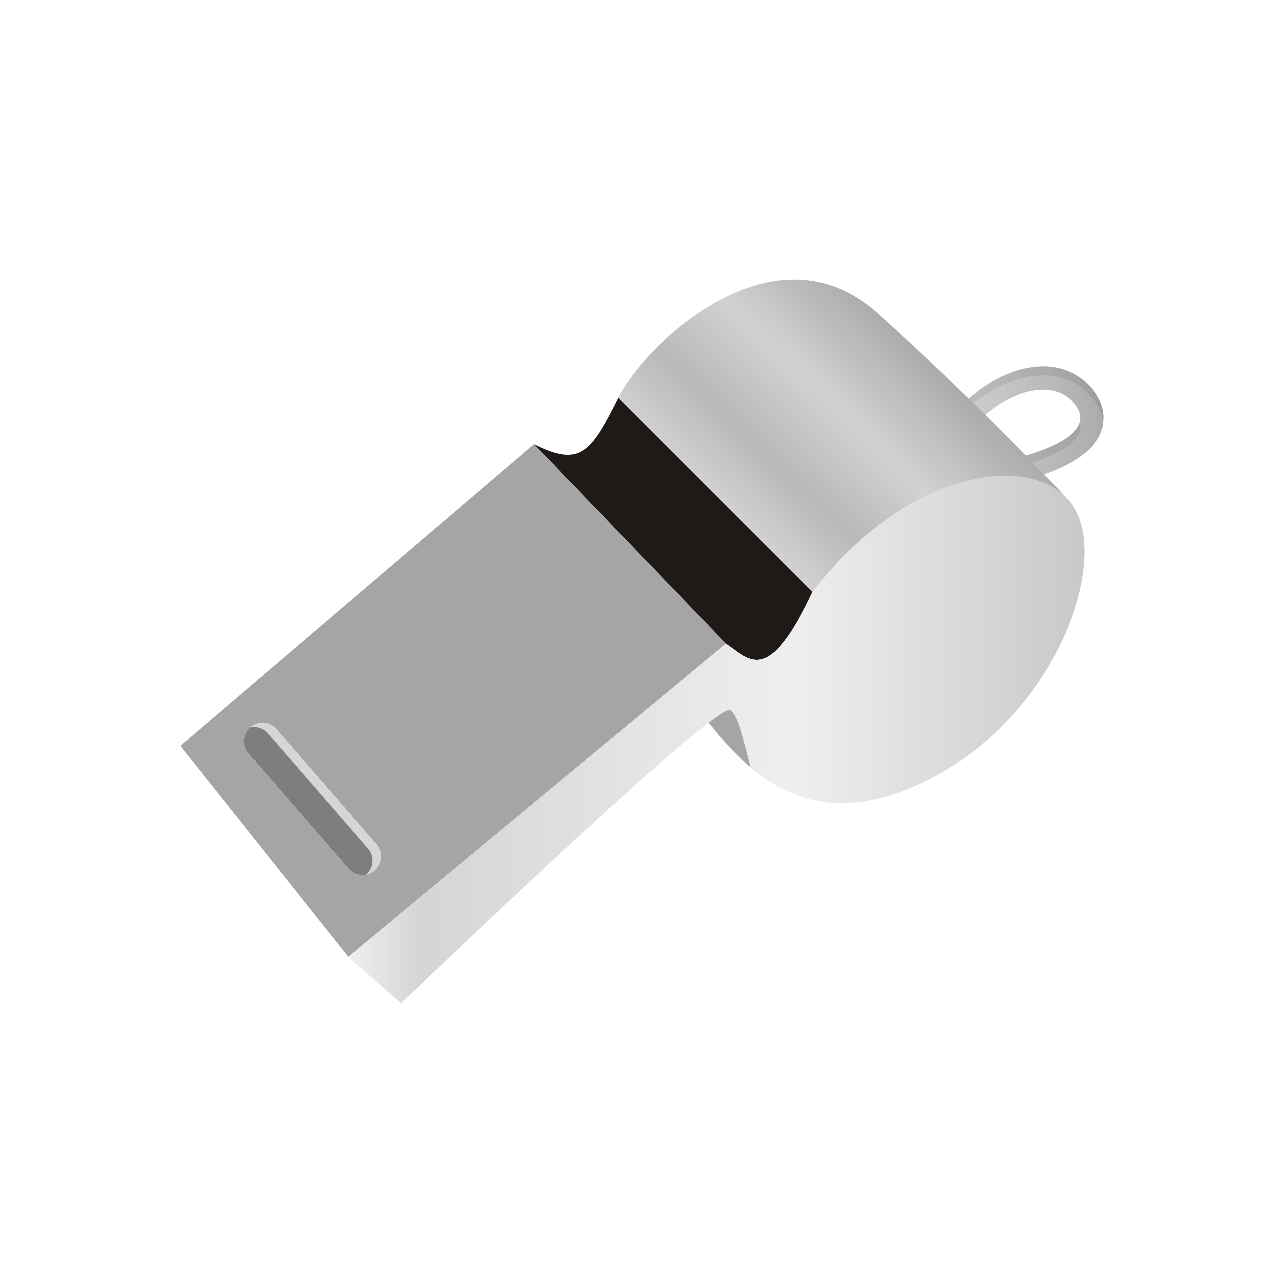
\includegraphics[width=0.250\textwidth]{sections/teoria/football-referee-whistle.eps}
\begin{figure}[!h]
\vspace{-10pt}
  \centering
    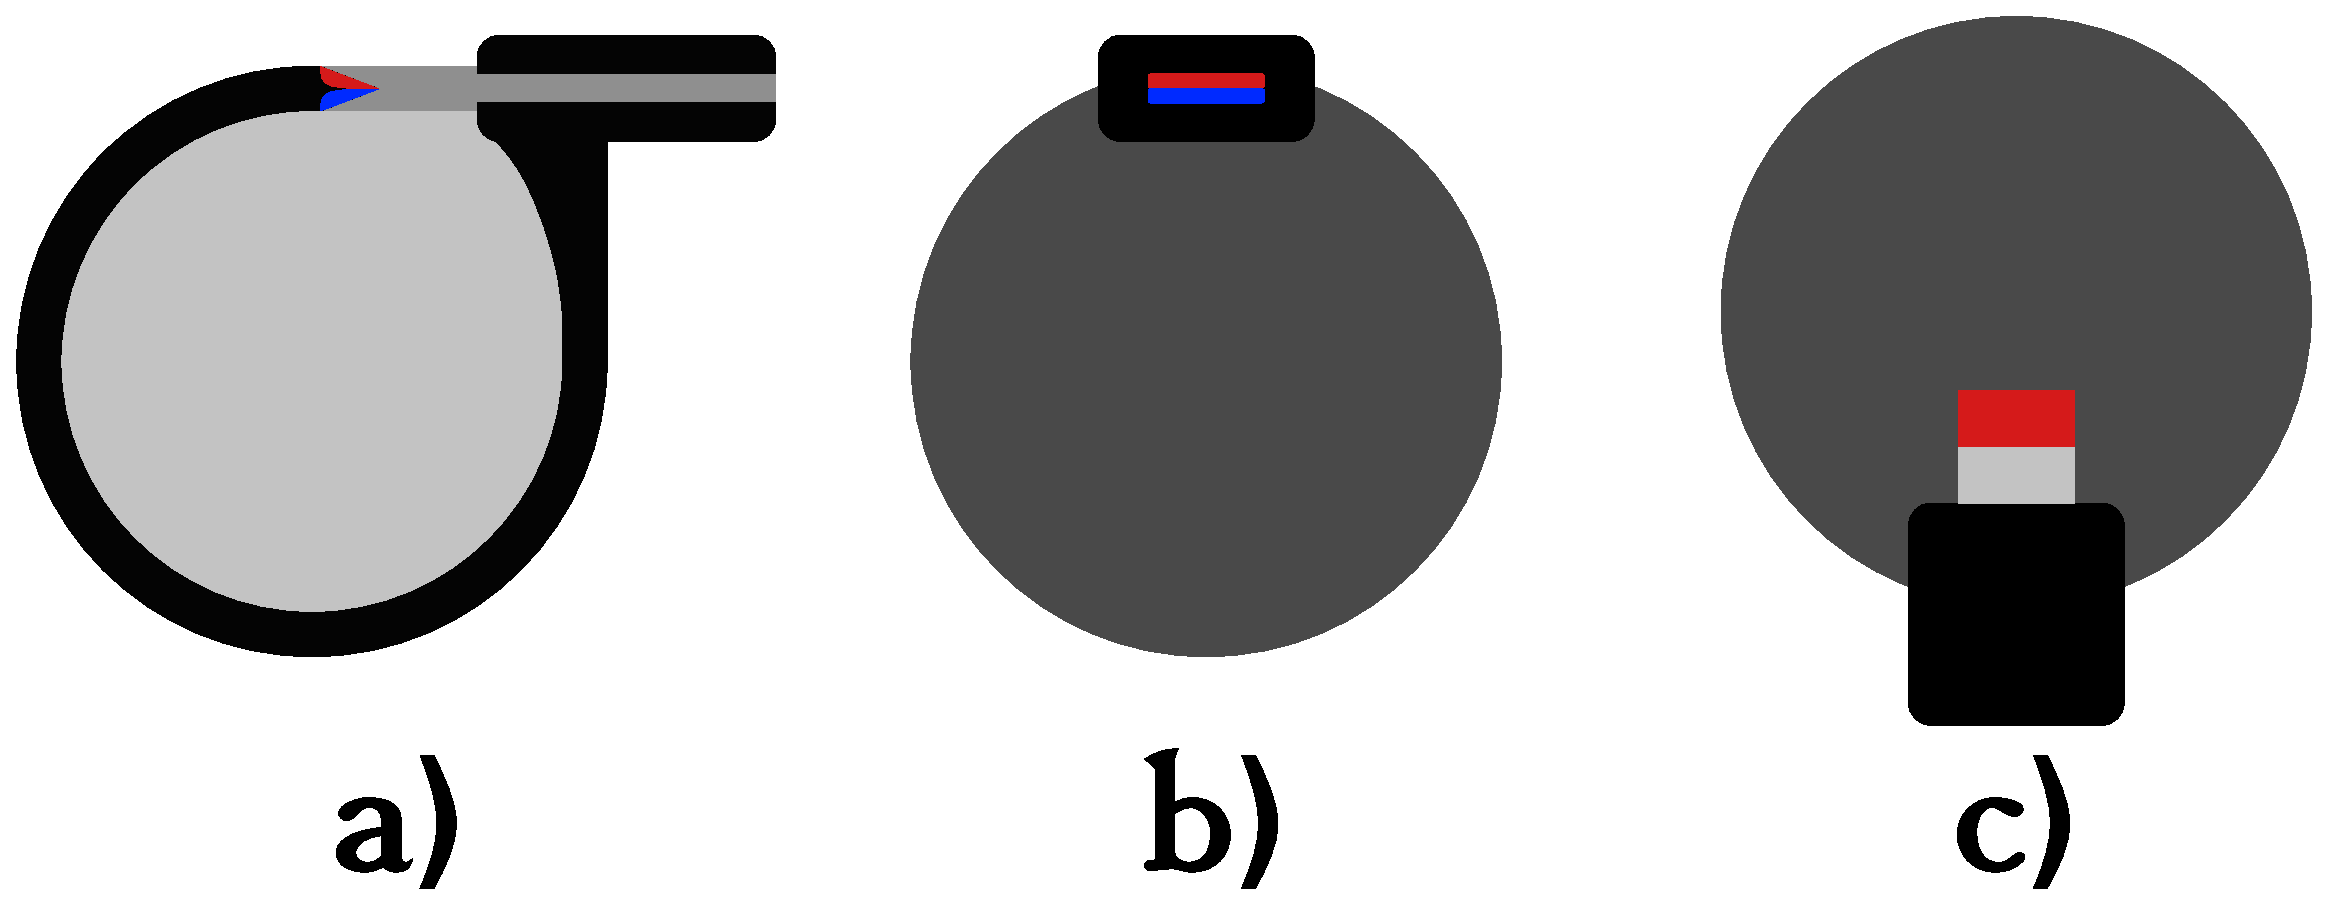
\includegraphics[width=0.950\textwidth]{sections/teoria/apito-vistas.eps}
\caption{Vistas de um apito.}
\label{fig:dinamica-energia-ex1}
\end{figure}
\end{frame}

%%%%%%%%%%%%%%%%%%%%%%%%%%%%%%%%%%%%%%%%%%%%%%%%%%%%%%%%%%%%%%%%%%%%%%%%%%
\begin{frame}
\frametitle{Boca principal}
 \includegraphics[width=0.250\textwidth]{sections/teoria/furo-principal.png}
\end{frame}
